%%% Local Variables:
%%% mode: latex
%%% TeX-master: "../main"
%%% End:

%\chapter{外文资料原文}
%\label{cha:engorg}
%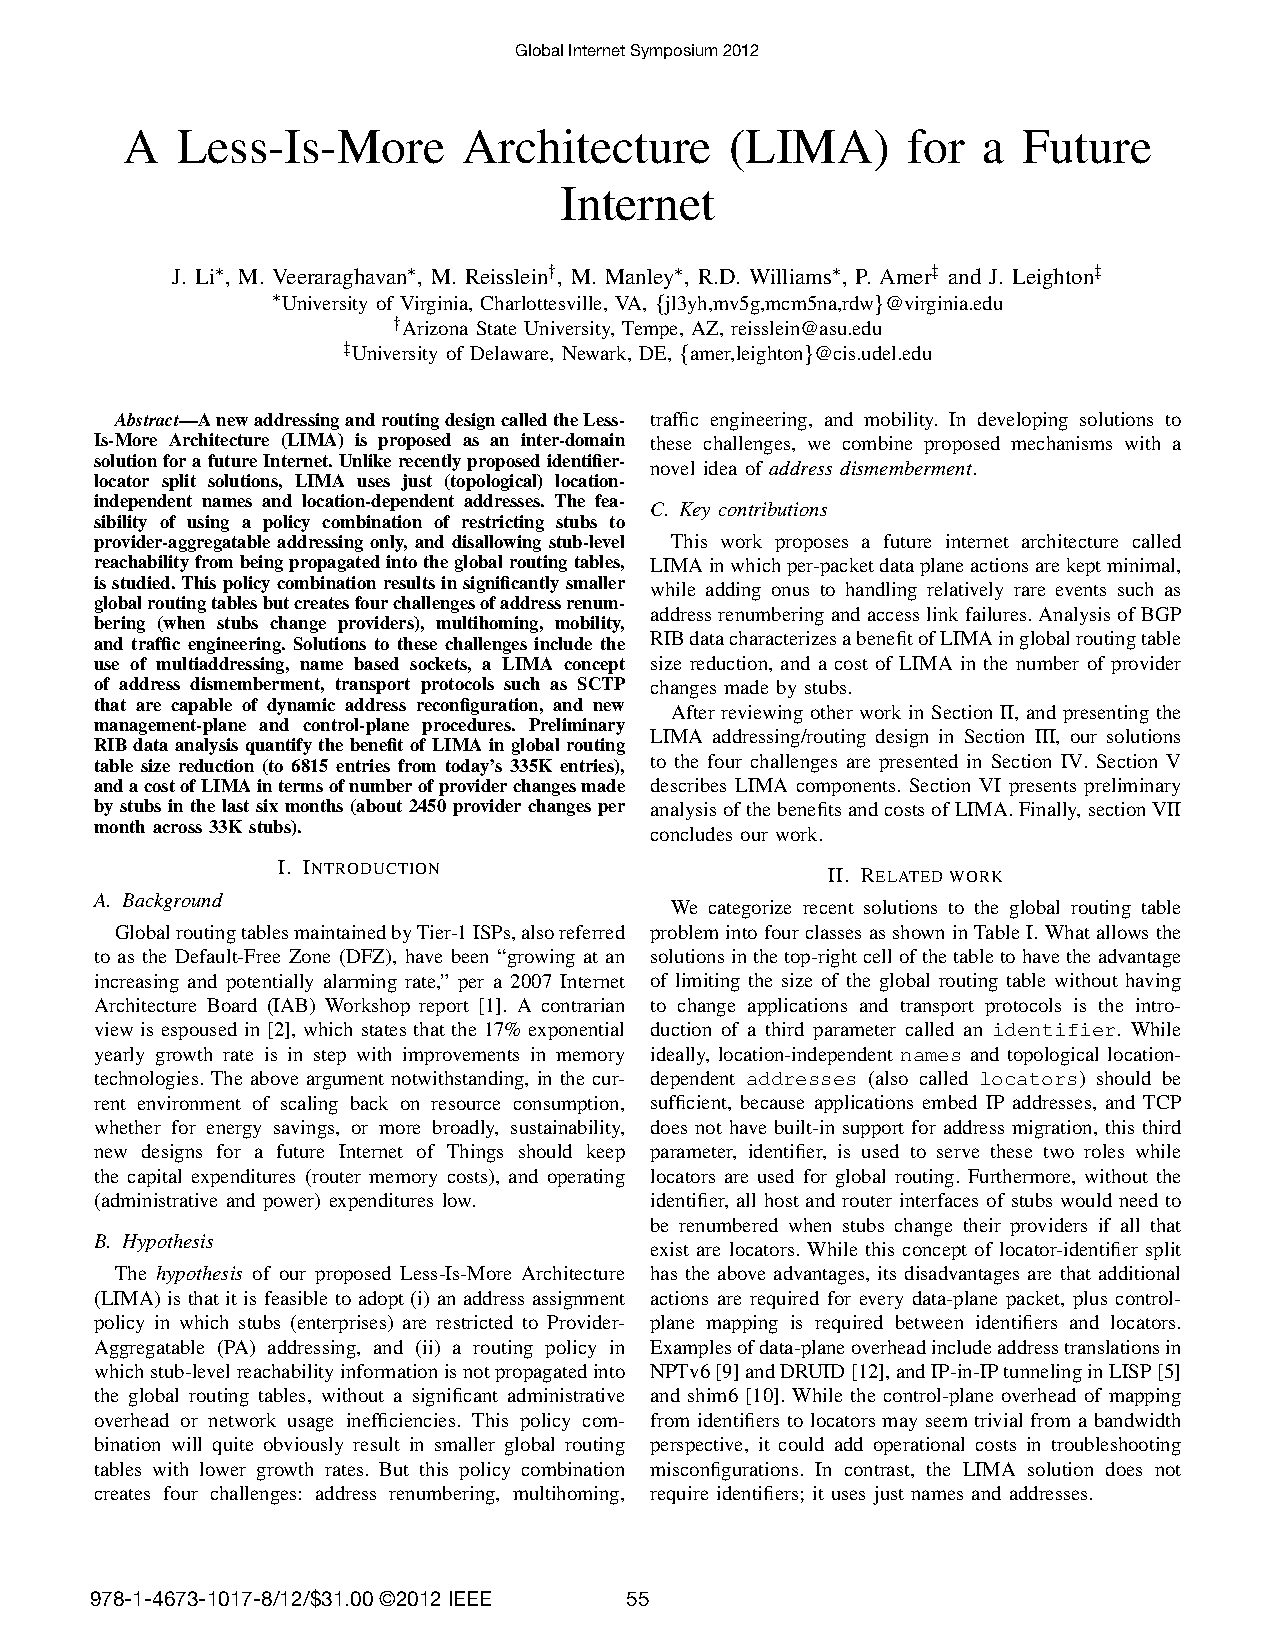
\includepdf[pages=1-6,turn=false]{ref.pdf}


\chapter{外文资料的调研阅读报告或书面翻译}

\textbf{未来互联网中的Less-Is-More结构\cite{lima}}

在未来互联网的发展中,人们提出了一种解决域间路由问题的新型寻址和路由设计,称之为Less-Is-More结构。该设计不同于最近提出的身份位置分离的解决方法,而是使用与位置无关的名称和与位置有关的地址。该设计需要结合两大相关政策,即stub必须是PA地址和stub级别的路由表信息不能扩散到全局路由表中。但政策的可行性还在研究中。该政策和设计的结合很大程度上导致全局路由表变小,但是也带来了四大挑战,即地址重编号(当stubs改变服务商),多宿主,移动性和流量工程。解决这些挑战的方法也有很多,比如使用多地址,基于端口的名字,LIMA概念的地址分解,特定传输协议(比如能够进行动态地址重配的SCTP协议),新的管理平台和控制平台程序。从基础的RIB数据分析可以确定LIMA结构可以将全局的路由表大小从现在的335K表项变成6815个表项。Stub的更新导致服务提供商的变化,维护LIMA结构的主要因素为服务提供商的改变,最近6个月平均每月有2450家服务商变化经过33k的stub。

I.	介绍\\
A.	背景\\
2007年,互联网构架委员会的一篇报告指出,全局的路由表由一级的互联网服务提供商维护,在默认的区域也同样适用的全局路由表,正在以一个逐渐增长的惊人的速率增长。与此同时,有人提出了一个相反的观点,17\%的指数年增长速率与内存技术的提高相一致。这个想法在现今为了节省能源,减少资源消耗的大趋势中,不能被接受。也就是说,在未来互联网中的设计,应该控制资本支出(路由器内存的花费)和操作支出(管理和控制)。


B.	假设\\
LIMS的假设是实行新的地址分配政策,在这个政策中,stub必须是PA地址,同时stub级别的可达信息不能传播到全局的路由表中,这不需要一个有意义的管理部门,如果传播到全局,网络使用效率将会很低。该政策很明显导致全局路由表更小,而且有更低的增长速度。但是这个政策带来了四个挑战:地址重编号,多宿主,流量工程,和移动性。解决这些挑战的方法正在发展完善中,文中的方法是将地址分解这个新颖的概念和提出的机制相结合。


C.	关键点\\
这篇论文提出名为LIMA的新型互联网结构,在这个结构中使用的数据包大小尽可能的最小,这给处理一些小概率的事件,比如地址重编号和连接链路失败,增加了负担。通过分析BGP RIB数据,我们发现LIMA结构有利于减小全局路由表的大小,而LIMA主要开销是随着stub变化服务提供商变化的数目的大小。
在浏览第二部分的相关工作之后,在第三部分描述了LIMA结构下的寻址和路由设计,第四部分解决LIMA结构带来的四个挑战,第五部分描述了LIMA的组件。第六部分对LIMA的优势和开销做了基本的分析。最后,第七部分总结了我们的工作。


II.	相关工作\\
我们把现在解决全局路由表存在问题的方法归为4类,如表1。表中右上角的方法使用了称为身份标识的第三个参数,该参数的加入使得不需要改变应用和传输协议,就可以减少全局路由表的大小。理想状况下,与位置无关的名字和与拓扑位置有关的地址足够了,因为应用中嵌套了IP地址并且TCP不支持地址迁移。当使用与拓扑位置有关的地址进行全局路由时,需要第三个参数,身份标识。如果所有存在的地址都是与拓扑位置相关的地址,一旦stub改变了自己的服务商,如果没有身份标识,所有的主机和stub 的路由接口都需要重编号。这种位置身份分离的概念有以上的优势,但也有自己的劣势。比如每个数据平台的包需要更多的空间放置额外的指令,也需要一个管理身份和位置映射控制平台。比如数据平台应该包括NPTv6和DRUID的地址翻译和在LISP和shim6中的IP-in-IP隧道。从带宽的角度看,控制平台中身份和位置的映射看起来十分琐碎,它需要增加对于错误配置的故障排除操作花费。相反,LIMA的解决方法不需要身份,只使用名称和地址。\\
LIMA的层次化寻址解决概念和平铺式寻址概念,比如ROFL,完全相反。层次化的寻址结构带来了很多问题,除了路径伸展、还有复杂管理系统、移动性和多宿主等等,都在这篇论文中有说明。

\begin{figure}
  \centering
  % Requires \usepackage{graphicx}
  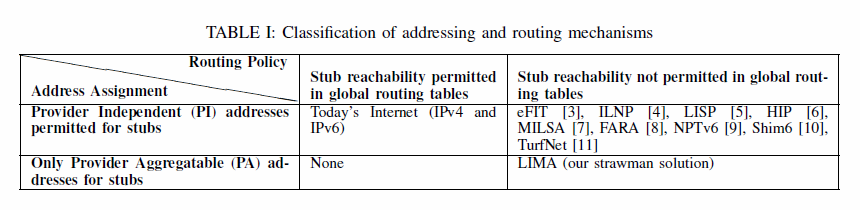
\includegraphics[width=\textwidth]{limatable1}\\
  \caption{寻址路由分类机制}\label{fig:limatable1}
\end{figure}

为什么我们的解决方案是“less-is-more”。 在第一部分B假设中提到的结合政策的LIMA和地址分解概念都能够用ipv6在网络层测试,因为ipv6支持我们设计最关键的一个需求,那就是支持多地址,我们可以通过多地址可以找到接口。LIMA是“less-is-more”,因为从现今的ipv6的解决方法角度考虑,这种方法去掉了ARP和最大长度匹配;从LISP和NPTv6的角度考虑,不需要翻译和隧道的支持;从NDN的角度考虑,NDN中的名字是基于每个包查找,NDN中使用160位地址的AIP协议,但LIMA要求更短的固定长度分解地址,比如说32位。为了避免每一包有更复杂的处理行为,LIMA对于额外的管理会做一个处罚,但仅限于地址重编号和多宿主stub中连接链路失败这两个小概率事件。暂且不论网络层,很多方面比如应用层,套接字接口,传输层协议,DHCPv6,DNS和BGP都需要做相应的变化为了支持LIMA结构,来解决该结构带来的四大问题。这些需要的变化正在当今互联网中慢慢进行。\\

III.	LIMA路由和寻址\\
LIMA主要是为了域间路由交流信息而设计的。具有额外的LIMA控制平台功能的Ipv6路由器将被使用在LIMA结构中。在该结构中,这些路由器的主要功能是作为域间路由器体现的,而不是域内路由器。在展示LIMA的寻址和路由之后,我们还讲述了两个域内stub网络的例子。\\
A.	寻址\\
简单来讲,LIMA的寻址是分层次的。这和ipv4/ipv6寻址有相似之处,需要一个全局路由前缀和一个接口身份标识,不同之处如下:

\begin{enumerate}
\item	使用自制系统号作为前缀
\item	给服务提供商分配的AS号必须是全局独一无二的AS号,而给stub分配的AS号是由它的服务提供商分配的本地服务商的AS号。这种方法不同于stub中可以在IP中使用PI地址。
\item   重新使用在域内路由网络中使用的地址作为接口身份标识,类似于ipv6地址可选选项中的MAC地址被扩展成EUI-64格式,然后被使用在interface-ID领域。
\end{enumerate}

第一个概念在参考文献第二篇中也被提及过。现今ipv4网络中前缀数目大约是335k,远大于服务提供商的AS号数目大约6185;第二个概念也在别的工作中出现过,比如eFIT,区分用户网络和服务商网络。尽管第一部分提到过,eFIT需要一个身份标识,而LIMA不需要。第三个概念和less-is-more的理念相一致,去掉了ARP和相关的安全威胁。虽然去掉了ARP,但是考虑到安全因素,我们提议在LIMA中使用DHCPv6,而不是SLAAC。MAC地址有时候是很私密的,因为它可以暴露NIC服务商的名字。如果使用动态赋值MAC地址就可以避免泄露MAC地址。为了避免欺骗,需要增加源地址过滤。


以上对LIMA寻址的描述,从IP寻址角度看,给读者提供了一个新的思路。基本的原理是把地址分成三个有区别的部分:全局独一无二的服务提供商AS号、本地服务商stub的AS号、本地stub域内地址。这三个部分对应到ipv6的地址结构上,前4个比特是全局独一无二的服务商AS号,接着4个比特是本地服务商stub的AS号,最后的8个比特是本地stub域内地址。L-DHCPv6和DNS需要进行修改来适应LIMA,L-DHPv6和L-DNS被用来标识LIMA版本的协议。一个服务商可以有多个AS号,一个服务提供商可以给它的stub分配多个AS号。


我们面临的一个问题就是如何区分一个组织是服务提供商还是stub。比如内容传送网络服务提供商:谷歌,雅虎,微软和Akamai,这些服务提供商并不能提供一条网络专线用于网路传输,现在他们的域名和很多的stub域相关联。类似的,一些客户互联网服务提供商不提供转发服务,不管是从他们的顾客来的起源和终结。我们可以通过一个给定AS的域间连接数目来区分该AS是一个服务提供商还是一个stub。这个问题在未来还可以继续研究。


B.	LIMA路由\\
LIMA路由不同于下面写的IP路由。在IP路由中,一级路由表的信息包括PI和多宿主PA stub,路由需要实现最大长度匹配。在LIMA中,一级路由表没有任何关于stub的消息,也没有最大长度匹配。相反,在LIMA中,在服务提供商网络边界路由器中的分离路由表中维护的信息是,服务商AS号和stub AS号。快速的并行查表可以通过硬件实现。当一个数据报到达目的服务商网络时,stub AS号表决定该数据报从哪个边界路由器出去。Stub边界路由器有两个表,当出口数据报经过边界路由器时,边界路由器查询服务商AS号路由表,当入口数据报进入有多个stub AS号的stub时,边界路由器查询stub AS号路由表。


C.	域内stub网络举例\\
接下来我们将通过两个域内stub的例子来说明分解寻址的概念:一个扁平化以太交换网络和一个层次结构私有ipv4路由网络。在以太网案例中,IDA就是MAC地址。我们曾经提出给L-DHCPv6服务器赋动态的MAC地址,为了强度更大的资产管理。另外,在初始化的时候,L-DHCPv6服务器要发送 { 服务提供商AS号,stub AS 号 } 对给终端。L-DHCPv6客户端在考虑地址分解的各个部分之后,在接口配置中创建他们的ipv6地址。在单个以太接口的一个多宿主stub中的一台的主机将有一个单一的IDA(MAC地址)。用MAC地址联系多对 { 服务提供商AS号, stub AS 号}产生多个ipv6地址。类似,在一个层次结构私有ipv4路由网络中的stub将会使用私有ipv4地址作为IDAs,写在ipv6地址的ID区域。


每一个主机接口对应一个权威的与IDA相关的名字。另外,一个名字对应一个主机,匹配多个接口对应的多个权威的名字。L-DNS服务器会存储所有终端名字与IDA的映射和一些简单的入口映射从组织名字映射到 { 服务提供商AS号, stub AS 号 }对。一个完全符合规定的主机域名需要结合带有主机名的组织名字。L-DNS的查询和安全动态DNS更新支持分解地址结构,可以使用stub名字或者一个特殊的终端名字。


IV.	设想的四种挑战的解决方法地址重编号


A.	地址重分配 \\

为了彻底实现全自动重新编号,LIMA采用参考资料[17],[18]的机制,该机制可以分为三类:(i)主机相关,(ii)DNS相关,(iii)路由器相关。


主机相关。关键的特征包括:(a)多地址寻址,(b)基于端口的名字(NBS)[19](c)地址分解的LIMA概念(d)SCTP[20]和MPTCP[21]的使用。多地址对带有停工的地址重编号至关重要,因为当在执行地址重编号的所有步骤中,stub能维护与旧服务提供商的连接信息1到2天。 然后,要求应用只能使用域名,避免使用NBS在应用中缓存任何地址的情况,应用对于NBS都应该是很灵活的。应用只存储或者处理名字,NBS层将名字翻译成地址。再者,地址重分配需要把新的 { 服务提供商 AS 号, stub AS 号}对广播给stub里面的所有终端,L-DHCPv6客户端收到发过来的参数,结合没有变化的IDAs生成ipv6地址,配置接口。最后,因为大部分的TCP连接都是短暂的,而且与旧服务商的连接需要每过一段时间进行维护,以防DNS缓冲查询区的数据失效,所以基于地址的一些旧的服务器不再使用后,某些连接需要终止。如果是长期的TCP连接,支持动态地址重配的传输层协议发生类似的情况,就重新连接。为了支持这个结构,我们提出使用SCTP和MPTCP。


DNS相关。接下来,让我们研究一下DNS的更新和DNS的缓存。现在的DNS服务器对每一个域名都维护一个完整的IP记录。在LIMA中,我们把数据库的每一条记录改为组织名(比如: Virginia.edu)对应一个或者多个 { 服务提供商AS号, stub AS 号 } 对,存在单个的记录匹配主机的名字和IDAs。这样的结构更容易应对服务提供商的变化。为了让缓存区DNS记录在其他stub和服务供应商中使用,stubs要维护和旧服务提供商之间的连接长达最大生存时间。

路由器相关。我们认为一个LIMA路由控制器需要运行(i)L-DHCPv6客户端,(ii)一个L-DNS客户端,(iii)拥有一个标识性的路由接口。LIMA的分解地址将采用发展比较完善的自动路由配置技术,比如Netconf。隧道配置应用应该采用名称而不是IP地址。LIMA的分解地址也需要最新的防火墙过滤技术。


B.	多宿主 \\
图一展示了在LIMA政策下,当stub收到来自每一个服务提供商的本地服务提供商stub的AS号通过其服务提供商构造的{ 服务提供商AS号, stub AS 号 } 映射对,比如A-2和B-1。如果stub和服务商A的连接断开了,考虑LIMA的路由政策的限制,一级互联网服务提供商不能到达A-2,结果没有数据包通过服务商B到达A-2。对于这个问题,我们提出了一个解决方法,那就是在stub的边界路由器和服务商A的边界路由器之间建立一条通过服务商B的隧道(图1中的点虚线),然后我们就可以把这条隧道作为stub和服务商A之间的备用链路。理论上应该规定隧道的优先级来保护经过服务商B的连通链路。在BGP中MED值可以用来设置直接连接链路作为第一选择,将备用链路作为第二选择,当链路失败时使用备用链路。


为了数据报无中断转发,有三点要求。第一,当收到路由器发来的SNMP表明直接链路连接断开的信息,为了防止使用A-2地址进行新的连接,stub的错误管理系统告诉L-DHCPv6服务器,它会发出广播信息警示所有的终端停止使用A-2全局地址。第二,错误管理系统也应该通知L-DNS服务器(LIMA版本的DNS服务器),让它不要提供A-2地址的查询结果。第三,对于正在进行的连接,终端上面的L-DHCPv6客户端应该开始SCTP或者MPTCP动态地址重配。

\begin{figure}
  \centering
  % Requires \usepackage{graphicx}
  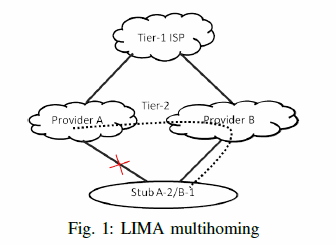
\includegraphics[width=\textwidth]{limafig1}\\
  \caption{LIMA 多宿主结构图}\label{fig:limafig1}
\end{figure}

C.	移动性\\
未来互联网设备中占据很大比例的可能是无线设备。其中,很大部分是移动,其中漫游比例可能较小。我们认为在LIMA层次化结构中,使用现今移动IP的方法来解决设备移动性的问题。


然而,为了减少路径扩展问题,我们建议结合动态DNS解决方法来增强移动IP的解决方法。现在有很多的方案提出使用安全动态DNS更新的结构来处理移动位置的管理,比如参考资料的[23],[24]。LIMA也使用了这样的方案。在LIMA中启用DNS服务器是非常有用的,因为这样当一个服务商改变的时候,stub的DNS服务器会告诉它的漫游设备,它本地发生了一些变化{ 服务提供商AS号, stub AS 号 }。在LIMA中使用移动IP可以处理DNS缓冲池中地址初始化时的连接,此外,本地stub边界路由器对它所有的终端支持本地代理,对游客支持外地代理。


D.	流量工程\\
与服务提供商相关的流量工程。在LIMA中取消现在符合ASN标准的前缀和最大前缀匹配,还有其路由政策中不允许stub的信息传到全局路由表,这些都可以导致路径延伸。比如两个主干路由器,Internet2和ESnet 。这两个路由器在洛杉矶、西雅图、芝加哥、纽约、华盛顿相互连接。ESet有两个stub客户,一个在加利福尼亚(CA),另一个在纽约(NY)。如果stub的信息可以传播出去,ESet能把它的两个stub的更长前缀匹配通知给Internet2 。从Internet2中美国堪萨斯州的路由器发给ESnet中美国加利福尼亚的包,在Internet2中将会向西朝着西雅图的路由器向前发包,如果这个包是发往美国纽约的路由器,那这个包将会往相反的方向朝着芝加哥路由器向前发包,前提条件是对于每一个路由器,在BGP更新时,都会收到来自不同路由器的信息,ESnet将会配置不同的MED值。但是,在LIMA中如果ESnet只能广播一个服务商AS号,这么有效的路由不能实现。


我们提出的解决方法是一个服务商有多个AS号,使得可以通过不同的AS号定位到这个服务商网络的不同地方。未来的工作中将会具体分析,为了实现好的交易,分配的AS号要尽可能的少,为了在低路径扩展值的情况下,不增加全局路由表的大小。


与Stub相关的流量工程。在当今的互联网中,为了平衡通过stub服务商的入口流量,一个多宿主的stub通过它的每一个服务商,有选择性地将更长前缀匹配的地址发给全局路由表。但在LIMA中,这是不可能的。我们提出了一个基于DNS和DHCP的方法来解决stub的流量工程问题。当应用程序请求选择地址的时候,stub权威的DNS服务器能整理多个地址将其返回给应用程序。对于出口流量,当告知stub的所有终端{ 服务提供商AS号, stub AS 号 }对,L-DHCPv6客户端使用不同的次序,同时用NBS层选择地址。


V.	LIMA组成部分\\
图二展示了由基于LIMA的边界ipv6路由器组成的stub网络的内部结构。使用NBS接口而不是TCP或者UDP接口修改应用。NBS为了调用套接字定义了一个新的本地类型AF\_NAME。接收方的listen和accept调用,发送方的open调用都是用域名而不是IP地址。Read和Write系统调用是NBS套接口描述器的接口函数。源地址信息放置在发送给目的地址的第一个ipv6扩展包中,接收应用会用名字而不是IP地址缓存关于源的信息(比如:颁发许可证的服务器)。


除了为了支持LIMA的分解结构而修改DHCPv6,地址重编码或者发生连接线路失败时,需要进行强制广播操作。不能使用DHCPv6重配消息,因为这个消息是用来重配一个简单的客户端的,而我们需要一类消息是stub中对所有全局地址可达终端加入或者删除{ 服务提供商AS号, stub AS 号 }对的命令。对于L\_DHCPv6服务器发送stub边界路由器接口的IDAs(也就是当今网络中的网关地址)和DNS服务器的IDA(现今DNS服务器的完整IP地址需要发给DHCP客户端)是非常高效的。因为LIMA比现在的网络更加依赖域名,预计来源于DNS客户端运行在终端上的安全动态DNS更新发生更加频繁,如图二。如果新的主机没有权威DNS更新要求的证书,L-DHCPv6服务器将会返回初始注册名字和IDA匹配。该行为要求在DHCPv6消息中增加名字。


需要对DNS进行简单地修改来适应地址分解结构。比如,原来数据库的结构应该修改成在第四部分A中提到的结构。一个自制系统地资源记录和对移动性的支持也应该加进去。
在处理链路连接失败的时候,要求LIMA错误管理系统与L-DHCPv6和L-DNS服务器通过一个协议相连接,如图2。在初始化和服务商改变的过程中,LIMA路由控制器支持路由接口的地址重分配。


为了支持LIMA的地址重分配,预计BGP也会做相应的修改。因为stub的AS号是本地服务商下的AS号,所以当BGP的更新和stub的AS号相关,stub边界路由器不仅要更新,stub的服务商边界路由器也要更新,而且服务商的AS号需要在服务商之间传播。

\begin{figure}
  \centering
  % Requires \usepackage{graphicx}
  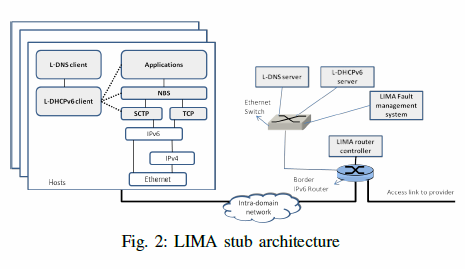
\includegraphics[width=\textwidth]{limafig2}\\
  \caption{LIMA stub结构图}\label{fig:limafig2}
\end{figure}

VI.	分析\\
评估LIMA需要几种不同的分析和原型结构,在这篇基础研究中,我们进行了两大分析。该部分A中验证使用LIMA降低全局路由表大小减少方面的优势,B中概括了地址重分配的评估。


A.	路由数据分析\\
通过分析近十年的路由器RIB数据,我们可以绘制AS总数、stub的AS数目和服务商AS数目的增长曲线,如图三。在LIMA中,全局路由表随着服务商AS的信号低速增长,现今共有6185个服务商。和335K的前缀和17\%的指数级年增长比率形成反差。

\begin{figure}
  \centering
  % Requires \usepackage{graphicx}
  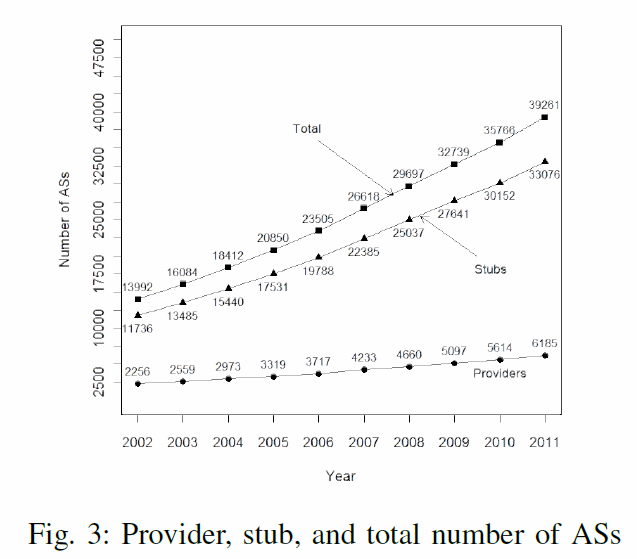
\includegraphics[width=\textwidth]{limafig3}\\
  \caption{LIMA Provider Stub AS总数}\label{fig:limafig3}
\end{figure}

B.	评估地址重编号\\
为了总结地址重分配花费代价的特征,我们分析了RIB数据为了确认stub增加或者删除服务商的频率,如表2。一些stub只增加或者减少服务商,但是增加或者减少服务商都能引起重编码操作,这两种情况都列在表2中。

\begin{figure}
  \centering
  % Requires \usepackage{graphicx}
  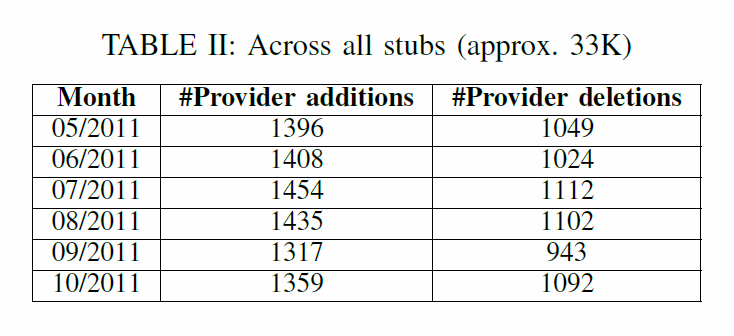
\includegraphics[width=\textwidth]{limatable2}\\
  \caption{服务商增加和减少数据}\label{fig:limatable2}
\end{figure}

图四绘制了与stub相关的每月服务商变化的平均数目,与前缀块大小的功能类似。前缀块越多,引发问题的可能性越大,即使地址重分配流程是完全自动的。随着时间的推移,总数在增长,但是比率恒定。比如,2011年和2002年,对于/24类型的stub服务商平均每月变化的数量是543和193。而2011年和2002年,stub的总数是29466和11250.因此,每个stub的服务商平均每月变化数目是2011年0.018,2002年0.017 。

\begin{figure}
  \centering
  % Requires \usepackage{graphicx}
  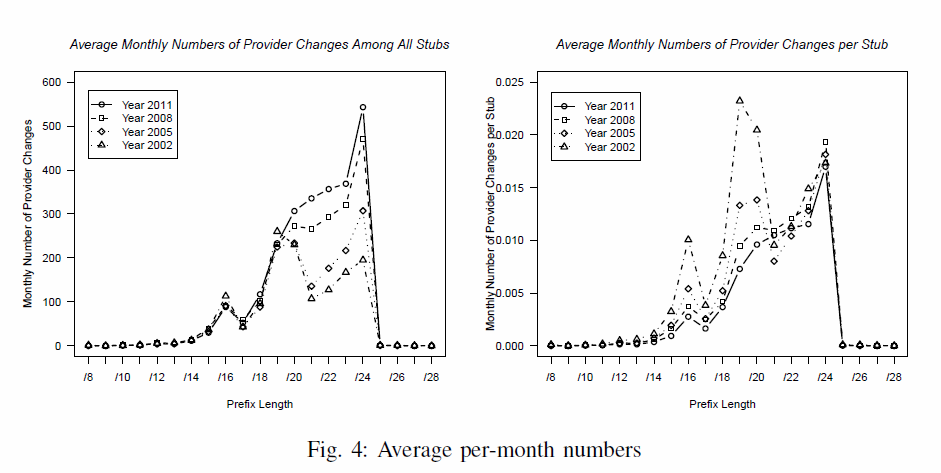
\includegraphics[width=\textwidth]{limafig4}\\
  \caption{stub相关的每月服务商变化的平均数目}\label{fig:limafig4}
\end{figure}


VII.	结论 \\
文中呈现的是一个完全地址分配和路由政策的结合,可能在今天的管理机构不流行,但是在处理地址重分配、多宿主、移动性和流量工程的问题中很灵活。相关的政策建议在stub上减少PI地址的使用,因为不允许stub级别的信息传到全局路由表中。在一个路由器比较多的stub中地址重分配在今天面临很大的挑战,需要有一些基础的改变,比如不允许在应用中使用IP地址而不是基于端口的名字,分解地址对于新的服务商AS号要做强制广播。和今天的IP相比,LIMA除了是更新的位置-身份分离方案,还按照比例缩减了每个包的指令(取消了最大长度匹配)。但是它增加了控制和管理平台,仅仅处理小概率事件,比如服务商改变和连接链路断开。LIMA 既减少了操作花费(管理和启动消耗),还通过降低内存和流程开销减少了资本支出。




%\chapter{其它附录}
%前面两个附录主要是给本科生做例子。其它附录的内容可以放到这里,当然如果你愿意,可
%以把这部分也放到独立的文件中,然后将其 \verb|\input| 到主文件中。
